\documentclass{beamer}

%\usetheme{Madrid}
%\usetheme{Boadilla}
%\usetheme{default}
%\usetheme{Warsaw}
%\usetheme{Bergen}
%\usetheme{Frankfurt}
\usetheme{Darmstadt}

\setbeamercolor{normal text}{fg=white}
\setbeamertemplate{background canvas}[vertical shading] [top=black!95,bottom=black!65]

\definecolor{mypurple}{RGB}{207,78,64}
\usecolortheme[named=mypurple]{structure}

\definecolor{myorange}{RGB}{255,235,190}
\beamerboxesdeclarecolorscheme{orange}{orange}{myorange}

\definecolor{commandcolor}{RGB}{111,195,165}

\setbeamertemplate{footline}[page number]
%\setbeamercovered{transparent}
\setbeamercovered{invisible}
\setbeamertemplate{navigation symbols}{}

%\usepackage{musixtex}
\usepackage{multimedia}
\usepackage{graphicx}
\usepackage[utf8]{inputenc}
%\usepackage[T1]{fontenc}
\usepackage[french]{babel} 
%\usepackage[all]{xy}
%\usepackage{multirow}
%\usepackage{lmodern}
\usepackage{subfigure}
%\usepackage{ulem}
\usepackage{url}
\usepackage{hyperref}
\usepackage{verbatim}
\usepackage{xspace}
\usepackage{color}
\usepackage{xcolor}
\usepackage{rotating}
\usepackage{multicol}
\usepackage[export]{adjustbox}
\usepackage{textpos}
\usepackage{listings}
\usepackage{fontawesome}


\definecolor{mypurple}{RGB}{207,78,64}
\usecolortheme[named=mypurple]{structure}

\definecolor{myorange}{RGB}{255,235,190}
\beamerboxesdeclarecolorscheme{orange}{orange}{myorange}

\definecolor{dgreen}{RGB}{0,125,0}

\usepackage{tikz}
\usetikzlibrary{trees}

\setbeamertemplate{caption}[numbered] 

\newcommand{\setframetitle}[1]{\begin{center}
    \huge \textbf{#1}
\end{center}}



\usepackage{chemfig}
\usepackage{rotating}


\usetikzlibrary{patterns}

\setbeamertemplate{caption}[numbered] 

\newcommand{\latex}{\LaTeX\xspace}

%% --------------

\title[Pr\'esentation de \latex]{D\'ecouverte de \latex}
\author{L\'eo \textsc{Baudouin}}
\institute{
  {\url{baudouin.leo @ gmail.com}}
}
\date{03-04 juin 2021}

%% --------------

\begin{document}

\begin{frame}
  \titlepage
\end{frame}

\begin{frame}
  \tableofcontents
\end{frame}

%% --------------

\section{Pr\'esentation}
\subsection*{}

\begin{frame}[fragile]
  \vspace{-5mm}
  \begin{center}
    \Huge \latex
  \end{center}

  \begin{center}
    \begin{minipage}{0.95\linewidth}
      \latex est un \emph{langage} et un \emph{système de composition} de documents créé en 1985. 
      Il fait partie de la famille des WYSIWYM\footnote{What You See Is What You Mean} et non de celle des WYSIWYG\footnote{What You See Is What You Get}, contrairement \`a Word ou OpenOffice.
    \end{minipage}
  \end{center}
  \vspace{2mm}

  \pause
  \hrule
  \vspace{5mm}
  Exemple :
  \begin{scriptsize}
\begin{verbatim}
  $\vec{a}$ est un vecteur, et $\left ( \begin{smallmatrix}
    a & b \\ c & d	%Superbe matrice
  \end{smallmatrix} \right )$
  est une            matrice.
\end{verbatim}
  \end{scriptsize}

  $\vec{a}$ est un vecteur, et $\left ( \begin{smallmatrix}
    a & b \\ c & d	%Superbe matrice
  \end{smallmatrix} \right )$
  est une            matrice.

\end{frame}

\subsection{Documents} 

\begin{frame}

  \begin{center}
    \Huge Documents \'ecrits
  \end{center}

  \begin{itemize}
  \item Rapport de stage
    \begin{itemize}
    \item \href{run:doc/RapportTechnique.pdf}{Rapport technique}
    \item \href{run:doc/RapportCulturel.pdf}{Rapport culturel}
    \end{itemize}
  \item Compte rendu
    \begin{itemize}
    \item \href{run:doc/CompteRendu.pdf}{Avanc\'ee d'un projet}
    \end{itemize}  
  \item Publication
    \begin{itemize}
    \item \href{run:./doc/Publi.pdf}{Recherche scientifique}
    \end{itemize}  
  \item \href{run:./doc/cv.pdf}{CV}
  \item Livre
  \end{itemize}
\end{frame}

\subsection*{Soutenances}
\begin{frame}
  \begin{block}{Exemple}
    Ceci est un exemple de soutenance
  \end{block}
  \begin{alertblock}{Mise en page}
    La mise en page est automatique.
  \end{alertblock}
  \pause
  \begin{exampleblock}{Animation}
    Possibilit\'e de faire de petites animations.
  \end{exampleblock}
\end{frame}

\subsection*{Compilation}
\begin{frame}

  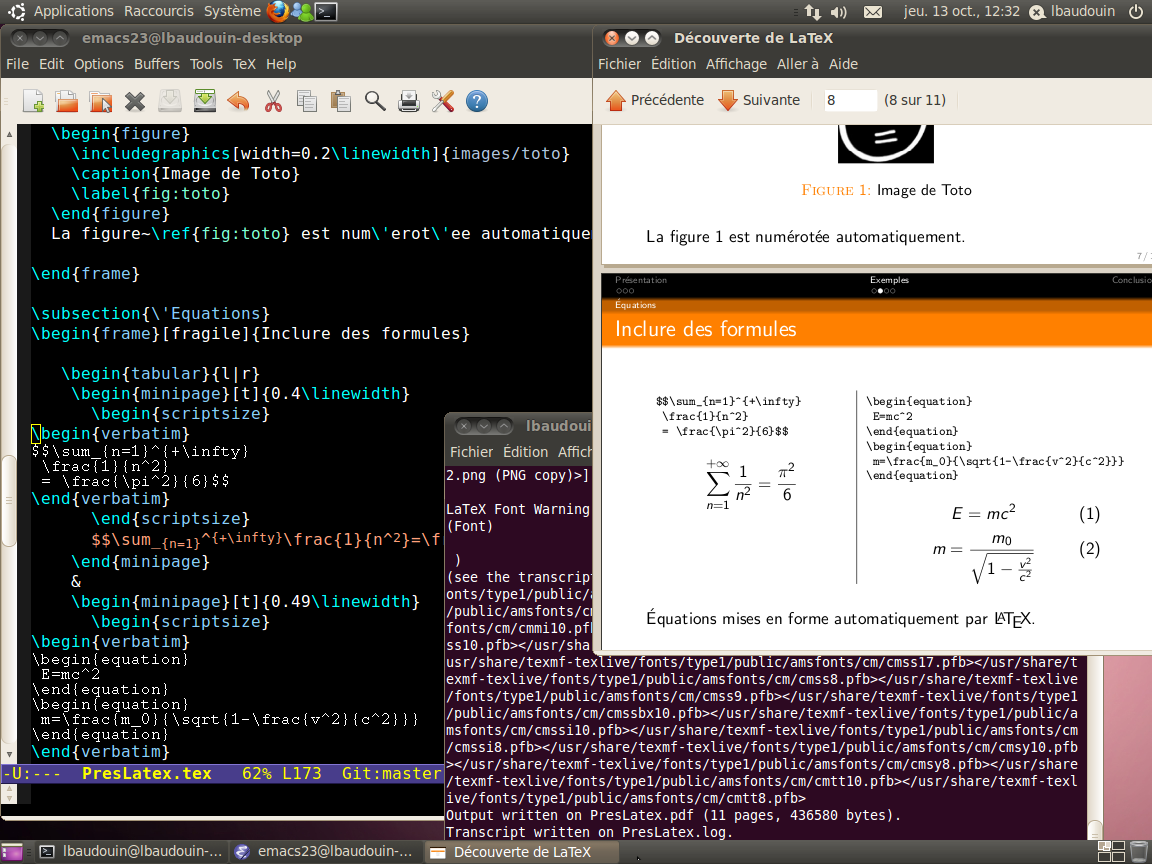
\includegraphics[width=0.95\linewidth]{images/Presentation}

\end{frame}

\subsection{Principe}
\begin{frame}[fragile]

  \begin{block}{Document minimal}
\begin{verbatim}
  \documentclass{article}
  \begin{document}
  Hello world!
  \end{document}
\end{verbatim}
  \end{block}
  \pause
  \begin{block}{Commande en ligne}
\begin{verbatim}
  {\it Texte.}
\end{verbatim}
  \end{block}
  \pause
  \begin{block}{Commande en bloc}
\begin{verbatim}
  \begin{center}
    Texte.                      
  \end{center}
\end{verbatim}
  \end{block}

  \pause
  
  \begin{block}{Fonctions}
\begin{verbatim}
  \textcolor{gray}{Texte en gris.}
\end{verbatim}  
  \end{block}
  
\end{frame}

\begin{frame}[fragile]
  \begin{block}{Utilisation de fonctions additionnelles}
\begin{verbatim}
\usepackage[utf8]{inputenc}  %Pour les accents
\usepackage[T1]{fontenc}     %Pour les fonts
\usepackage[french]{babel}   %Charge le Français
\usepackage{graphicx}        %Pour les figures
\usepackage{subfigure}       %Pour les sous-figures
\usepackage{hyperref}        %Pour les liens
\usepackage{verbatim}        %Pour écrire du LaTeX
\usepackage{xspace}          %Pour de bons espaces
\usepackage{tikz}            %Pour dessiner
\usepackage{color}           %Pour la couleur
\usepackage{chemfig}         %Pour la chimie
\usepackage{rotating}        %Pour tourner un peu tout
%...
\end{verbatim}
  \end{block}
\end{frame}

\subsection*{Conclusion}
\begin{frame}

  \begin{itemize}
  \item Avantages
    \begin{itemize}
    \item  \latex permet de cr\'eer n'importe quel type de document \'ecrit.
    \item Exporte les documents en \textit{.ps}, en \textit{.dvi}, mais surtout en \textit{.pdf}.
    \item Compatible Windows / Linux / Mac OS.
    \item Edition avec n'importe quel \'editeur de texte.
    \end{itemize}
    \pause  
  \item Inconv\'enients
    \begin{itemize}
    \item 1 \`a 2 semaines d'apprentissage.
    \item Obligation d'utiliser un compilateur (intégrer avec les IDE).
    \end{itemize}
  \end{itemize}
\end{frame}

%% --------------

\section{Exemples}
\subsection{Sommaire}

\begin{frame}[fragile]{Inclure un sommaire}
  \begin{tabular}{c | c}
    \begin{minipage}[c]{0.6\linewidth}
      \begin{figure}[b]
        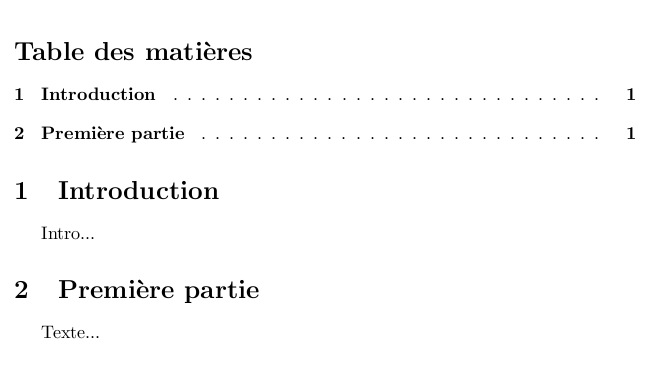
\includegraphics[width=\linewidth]{images/toc}
      \end{figure}
    \end{minipage}
    &
    \begin{minipage}[c]{0.35\linewidth}
      
      \begin{scriptsize}
\begin{verbatim}
  \tableofcontents
  \section{Introduction}
  Intro...
  \section{Première partie}
  Texte...
\end{verbatim}
      \end{scriptsize}
    \end{minipage}  \\ 
  \end{tabular}
\end{frame}

\subsection{Images}

\begin{frame}[fragile]{Inclure une image}

  \begin{small}
\begin{verbatim}
  \begin{figure}
    
\includegraphics[width=0.2\linewidth]{images/toto}
    \caption{Image de Toto}
    \label{fig:toto}
  \end{figure}
  La figure~\ref{fig:toto} est numérotée automatiquement.
\end{verbatim}
  \end{small}

  \hrule

  \begin{figure}
    
\includegraphics[width=0.2\linewidth]{images/toto}
    \caption{Image de Toto}
    \label{fig:toto}
  \end{figure}
  La figure~\ref{fig:toto} est numérotée automatiquement.

\end{frame}

\subsection{\'Equations}
\begin{frame}[fragile]{Inclure des formules}

  \begin{tabular}{l|r}

    %\onslide<1>{    
    \begin{minipage}[t]{0.4\linewidth}
      \begin{scriptsize}
\begin{verbatim}
  $$\sum_{n=1}^{+\infty}
  \frac{1}{n^2}
  = \frac{\pi^2}{6}$$
\end{verbatim}
      \end{scriptsize}
      
      $$\sum_{n=1}^{+\infty}\frac{1}{n^2}=\frac{\pi^2}{6}$$

    \end{minipage}
    %}
    &
    \begin{minipage}[t]{0.49\linewidth}      
      \begin{scriptsize}
\begin{verbatim}
  \begin{equation}
    E=mc^2                              
  \end{equation}
  \begin{equation}
    m=\frac{m_0}{\sqrt{1-\frac{v^2}{c^2}}}
  \end{equation}
\end{verbatim}

      \end{scriptsize}
      %  \onslide<2>{
      \begin{equation}
        E = mc^2                              
      \end{equation}
      \begin{equation}
        m = \frac{m_0}{\sqrt{1-\frac{v^2}{c^2}}}
      \end{equation}
      % }
    \end{minipage}
  \end{tabular}

  \vspace{5mm}
  \'Equations mises en forme automatiquement par \latex.\\
  Les équations peuvent être ajoutés dans le texte.\\
  L'équation deviendrait : $\sum_{n=1}^{+\infty}\frac{1}{n^2}=\frac{\pi^2}{6}$ (la police est plus petite).

\end{frame}

\subsection{Tableaux}
\begin{frame}[fragile]{Inclure un tableau}

  \begin{tabular}{c | c }
    \hspace{-5mm}
    \begin{minipage}{0.55\linewidth}
      \begin{scriptsize}
\begin{verbatim}
  \begin{tabular}{ | l | c || r | }
    \hline                       
    0      & 123       & $2\times2$\\
    blabla & 5         & 6 \\
    10     & $\vec{a}$ & 9 \\
    \hline  
  \end{tabular}
\end{verbatim}
      \end{scriptsize}
    \end{minipage}
    &
    \begin{minipage}{0.5\linewidth}
      \begin{center}
        \begin{tabular}{ | l | c || r | }
          \hline                       
          0      & 123       & $2\times2$\\
          blabla & 5         & 6 \\
          10     & $\vec{a}$ & 9 \\
          \hline  
        \end{tabular}
      \end{center}
    \end{minipage}
  \end{tabular}
\end{frame}

\subsection{Listes}
\begin{frame}[fragile]{Faire des listes}
  \begin{tabular}{c | c}
    \begin{minipage}{0.5\linewidth}
      Liste de points
      \begin{itemize}
      \item Item 1
      \item Item 2
      \item ...
      \end{itemize}
      
      Liste numérotée
      \begin{enumerate}
      \item Item 1
      \item Item 2
	\begin{itemize}
	\item Item 2.1
	\item Item 2.2	\end{itemize}
      \item ...
      \end{enumerate}
    \end{minipage}
    
    &
    \begin{minipage}{0.5\linewidth}
      \begin{small}
\begin{verbatim}
  Liste de points
  \begin{itemize}
  \item Item 1
  \item Item 2
  \item ...
  \end{itemize}
  
  Liste numérotée
  \begin{enumerate}
  \item Item 1
  \item Item 2
    \begin{itemize}
    \item Item 2.1
    \item Item 2.2
    \end{itemize}
  \item ...
  \end{enumerate}
\end{verbatim}
      \end{small}
    \end{minipage}
  \end{tabular}
\end{frame}
%% --------------

\subsection{Dessins}
\begin{frame}{Dessiner avec Tikz}

  \begin{center}
    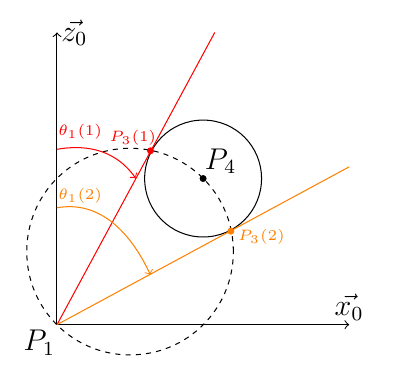
\includegraphics[width=0.31\linewidth]{images/dessin1}
    ~
    \href{http://www.texample.net/tikz/examples/three-link-annotated/}{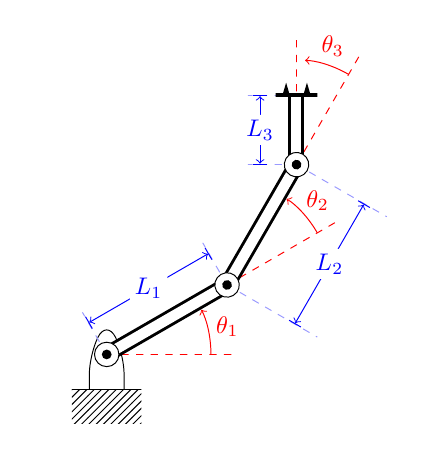
\includegraphics[width=0.31\linewidth]{images/dessin2}}
    ~
    \href{http://www.texample.net/tikz/examples/focused-ion-beam-system/}{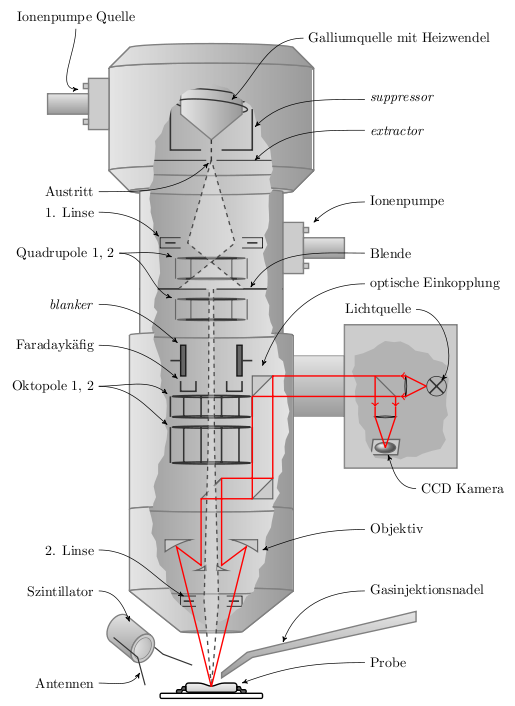
\includegraphics[width=0.31\linewidth]{images/dessin3}}
  \end{center}

  \begin{center}
    \small{ {\it Voir les codes correspondants \`a ces dessins sur \url{http://www.texample.net/tikz/}}}
  \end{center}
  
\end{frame}

\begin{frame}{Dessiner avec Tikz}
  \begin{center}
    \href{http://www.texample.net/tikz/examples/polarizing-microscope/}{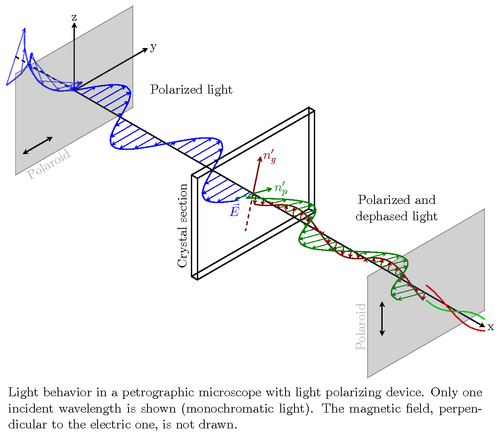
\includegraphics[width=0.48\linewidth]{images/schema}}
    ~
    \href{http://www.texample.net/tikz/examples/scientific-interactions/}{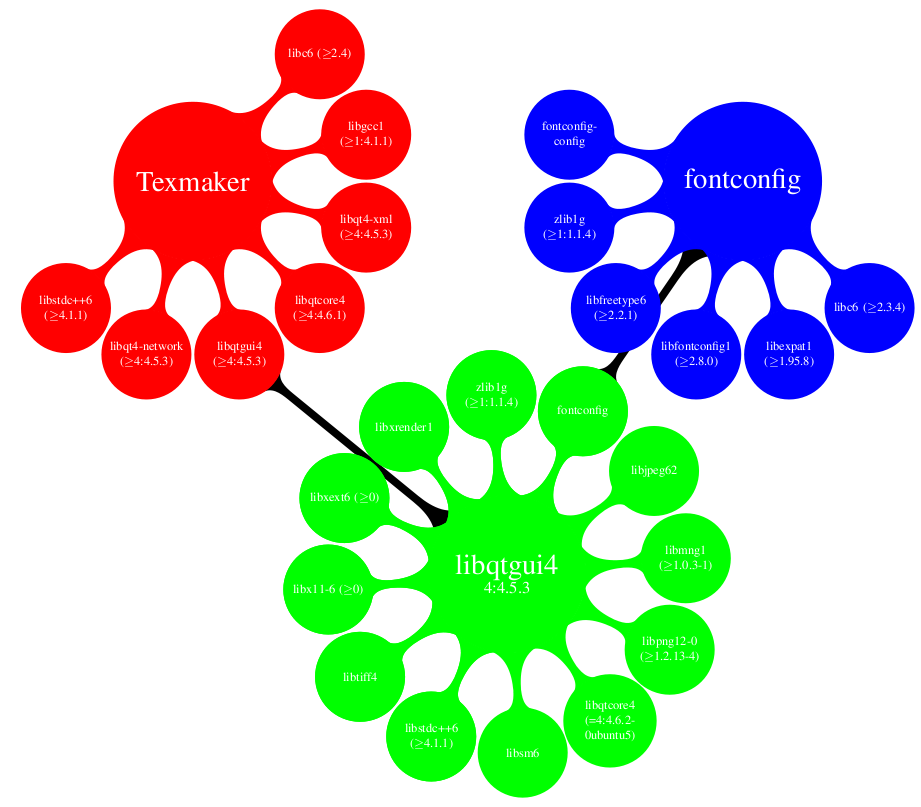
\includegraphics[width=0.48\linewidth]{images/depends}}
  \end{center}
\end{frame}

\subsection*{Musique}
\begin{frame}[fragile]{\'Ecrire une partition}

  \begin{tabular}{l|r}
    \begin{minipage}{0.6\linewidth}
      \begin{Tiny}
\begin{verbatim}
  \normalmusicsize 
  \begin{music} 
    \instrumentnumber{2} % 2 instruments
    \setstaffs 1{2} % instrument 1 (en bas) : 2 portées
    \setclef{1}{60} % clef de fa (6) en 1, clef de sol (0) en 2
    \generalmeter{\meterfrac{4}{4}} % mesure 4/4
    \setname 1{piano} %
    \setname 2{chant} %
    \parindent 10mm % pour éviter la collision de piano avec l'accolade
    \startextract
    
    \Notes 
    \ha J | % chgt portée, même instr
    \zhu{c e}\hu g & % chgt instr ; pas d'espace entre } et \hu
    \islurd0c\ibu0d0\qb0{c c c}\tslur0d\tbu0\qb0d 
    \enotes % assure l'alignement
    
    \Notes 
    \ha N | % chgt portée, même instr
    \zhu{g i}\hu k & % chgt instr
    \qa{e d} 
    \enotes 
    \bar % après toutes les notes de la mesure, pour toutes les voix
    
    \Notes
    \qa J | 
    \zqu{c e}\qu g &
    \islurd0c\ibu0d0\qb0{c e} 
    \enotes
    
    \Notes
    \qa N |
    \zqu{g i}\qu k &
    \qb0{d}\tslur0d\tbu0\qb0d
    \enotes
    
    \Notes
    \ha J | 
    \zhu{c e}\hu g &
    \ha c 
    \enotes
    \endextract
  \end{music}
\end{verbatim}
      \end{Tiny}
    \end{minipage}
    &
    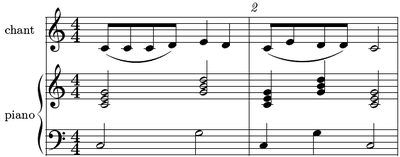
\includegraphics[width=0.4\linewidth]{images/MusixTex}
  \end{tabular}
\end{frame}


\subsection*{Chimie}

\begin{frame}[fragile]{\'Ecrire de la chimie}

  \begin{tabular}{l|r}
    
    \begin{minipage}{0.45\linewidth}
      \begin{scriptsize}
\begin{verbatim}
  \chemfig{H-\chemabove{N}
    {\scriptstyle\oplus}(=[1]O)-
    [7]O^{\ominus}-*6(=-=-=-)}
\end{verbatim}
      \end{scriptsize}
    \end{minipage}
    &
    \chemfig{H-\chemabove{N}{\scriptstyle\oplus}(=[1]O)-[7]O^{\ominus}-*6(=-=-=-)}
  \end{tabular}

\end{frame}

\subsection{Bibliographie}
\begin{frame}[fragile]
\begin{block}{Citation}
\begin{verbatim}
  \cite{Chestnutt:ICRA:2005}
\end{verbatim}
\end{block}

\begin{block}{Inclure la bibliographie}
\begin{verbatim}
  \bibliography{./IEEEabrv,./main}
\end{verbatim}
\end{block}

\begin{block}{Bibliographie}
\begin{tiny}
\begin{verbatim}
  @InProceedings{ baudouin:humanoids:11,
	author = "L. Baudouin and N. Perrin and O. Stasse and T. Moulard and E. Yoshida and F. Lamiraux",
	title = "{R}eal-time {R}eplanning {U}sing 3{D} {E}nvironment for {H}umanoid {R}obot",
	booktitle = "IEEE Int. Conf. on Humanoid Robotics (Humanoids'11)",
	year = "2011",
	note = "submitted"
  }
\end{verbatim}
\end{tiny}
\end{block}

\begin{block}{Gestion de la bibliographie}
\begin{itemize}
\item kbibtex
\item jabref
\item Mendeley
\end{itemize}
\end{block}

\end{frame}

\subsection{Personnalisation}
\begin{frame}[fragile]
  \begin{block}{Commandes}
\begin{verbatim}
\newcommand{\leo}{L\'eo B\textsc{audouin}\xspace}
\end{verbatim}
  \end{block}

  \begin{block}{Fonctions}
\begin{verbatim}
\newcommand{\smallfig}[4]{
  \begin{figure}[h]
    \begin{center}
      \includegraphics[width=#1\linewidth]{#2}
      \caption{#3}
      \label{#4}
    \end{center}
  \end{figure}
}
\end{verbatim}
  \end{block}

\end{frame}

%% --------------

\section{Conclusion}
\subsection*{}
\begin{frame}{Conclusion}

  \begin{center}
    {\huge \latex}\\
  \end{center}

  \begin{enumerate}
  \item Alternative int\'eressante aux \'editeurs de documents habituels 
  \item Tr\`es performant pour les documents scientifiques
  \item Tr\`es utile pour les documents litt\'eraires
  \item Mise en page automatique
  \item Rendu vectoriel
  \item Nombreux wikis\footnote{\url{http://fr.wikibooks.org/wiki/LaTeX}} d'aide
  \item Nombreux tutoriels\footnote{Le site du zéro / openclassroom}
  \end{enumerate}

\end{frame}


\subsection*{\`A vous de jouer}
\begin{frame}[fragile]{Installation}

  \begin{itemize}
  \item Windows
    \begin{itemize}
    \item TexLive : \url{http://www.tug.org/texlive/}
    \item MikTex : \url{http://miktex.org/}
    \end{itemize}
  \item Mac
    \begin{itemize}
    \item MacTex : \url{http://www.tug.org/mactex/}
    \end{itemize} 
  \item Linux
    \begin{itemize}
    \item TexLive : \verb+sudo apt-get install texlive+
    \end{itemize}
  \item Choisir un editeur de texte
    \begin{itemize}
    \item \textbf{TexMaker} : \url{http://www.xm1math.net/texmaker/}
    \item LyX : \url{http://www.lyx.org/}
    \item Kile : \url{http://kile.sourceforge.net/}
    \item TeXnicCenter : \url{http://www.texniccenter.org/}
    \item Online : \url{https://www.overleaf.com/}
    \item Emacs / vi / Bloc-note / \dots
    \end{itemize}
  \end{itemize}
\end{frame}

\subsection*{Exemple}

\begin{frame}[fragile]{Exemple}
      \begin{itemize}
      \item Item normal
      \item[$\diamond$] Autre item
      \item[2012] Avec une date !
      \end{itemize}
\end{frame}


\end{document}  
